\documentclass{beamer}
%
% Choose how your presentation looks.
%
% For more themes, color themes and font themes, see:
% http://deic.uab.es/~iblanes/beamer_gallery/index_by_theme.html
%
\mode<presentation>
{
  \usetheme{default}      % or try Darmstadt, Madrid, Warsaw, ...
  \usecolortheme{default} % or try albatross, beaver, crane, ...
  \usefonttheme{serif}  % or try serif, structurebold, ...
  \setbeamertemplate{navigation symbols}{}
  \setbeamertemplate{caption}[numbered]
} 

\usepackage[english]{babel}
\usepackage[utf8]{inputenc}
\usepackage[T1]{fontenc}
\usepackage{graphicx}
\usepackage{subcaption}

\title[Your Short Title]{Supertasks}
\author{Vatsav Sethupathi}
\institute{University of Arizona}
\date{14th April 2020}

\begin{document}

\begin{frame}
  \titlepage
\end{frame}

% Uncomment these lines for an automatically generated outline.
%\begin{frame}{Outline}
%  \tableofcontents
%\end{frame}

\section{Introduction}

\subsection{A few points to note}

\begin{frame}{Things to note before beginning!}

\begin{itemize}
  \item I was inspired to explore this topic after watching a video on it by VSauce.
  \item Link to the video: https://www.youtube.com/watch?v=ffUnNaQTfZE
  \item This presentation explores the concept of supertasks using famous examples and thought experiments. 
  \item Let's begin!
\end{itemize}

\end{frame}

%\vskip 1cm

%\begin{block}{Examples}
%Some examples of commonly used commands and features are included, to help you get %started.
%\end{block}

\subsection{Though Experiment 1}

\begin{frame}{The first thought experiment (involves cake!)}
    \begin{itemize}
        \item Imagine you have a delicious cake in front of you, with a knife meant to cut the cake.
        \item Cut the cake in half.
        \item Now, cut one of the smaller halves of the cake in half once again.
        \item Continue this pattern and keep cutting one of the smaller halves again and again
        \item Simultaneously keep stacking these smaller pieces one on top of each other.
    \end{itemize}
    
    \begin{block}{}
    Can we make an observation about the structure we have created?
    \end{block}

\end{frame}

\section{Supersolids}

\subsection{What are Supersolids}

\begin{frame}{Supersolids}
    \begin{itemize}
        \item A supersolid is a geometric shape that has a finite volume, but an infinite surface area.
    \end{itemize}
    
    \begin{figure}[h]
        \centering
        \begin{subfigure}[b]{0.4\linewidth}
            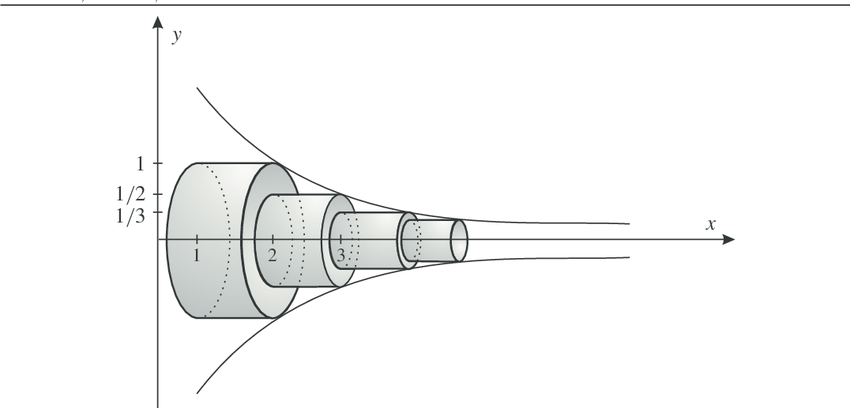
\includegraphics[width=\linewidth]{cake.png}
            \caption{A picture of the cake in we discussed above}
        \end{subfigure}
        \begin{subfigure}[b]{0.4\linewidth}
            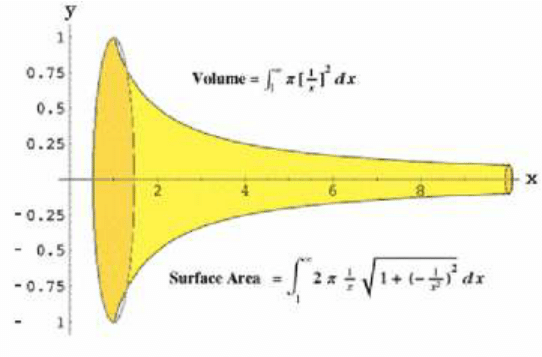
\includegraphics[width=\linewidth]{horn.png}
            \caption{Another supersolid that we will be discussing}
        \end{subfigure}
        \caption{Examples of supersolids}
        \label{fig:coffee}
    \end{figure}

\end{frame}

\subsection{Gabriel's Horn}

\begin{frame}{Gabriel's Horn}

    \begin{figure}
        \centering
        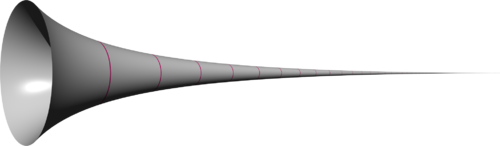
\includegraphics[width=\linewidth]{horn1.png}
        \caption{Gabriel's Horn}
        \label{fig:my_label}
    \end{figure}
    \begin{itemize}
        \item This is a supersolid that is based on the graph of $\frac{1}{x}$
        \item The name refers to the Abrahamic tradition identifying the archangel Gabriel, associating the divine, or infinite, with the finite.
        \item It is also referred to as Toricelli's Trumpet since the properties of this figure were first studied by Italian physicist and mathematician Evangelista Torricelli in the $17^{th}$ century.
    \end{itemize}
\end{frame}

\begin{frame}{Mathematical Representation of Gabriel's Horn (1/2)}
\begin{figure}[h]
    \centering
    \begin{subfigure}[b]{0.4\linewidth}
      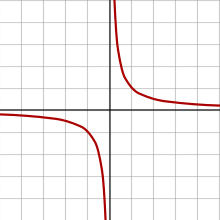
\includegraphics[width=\linewidth]{Graph 1.png}
      \caption{2D Graph of $\frac{1}{x}$}
    \end{subfigure}
    \hspace{4mm}
    \begin{subfigure}[b]{0.4\linewidth}
      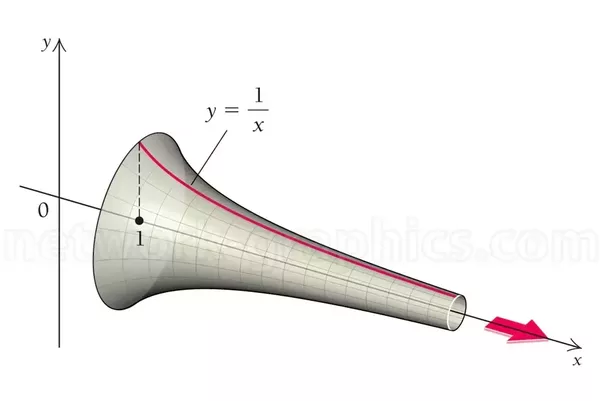
\includegraphics[width=\linewidth]{Graph 2.png}
      \caption{Graph of $\frac{1}{x}$ rotated along x=0}
      \begin{minipage}{.1cm}
      \vfill
      \end{minipage}
    \end{subfigure}
    \caption{The graphs of $\frac{1}{x}$ in 2 and 3 dimensions}
    \label{fig:my_label}
\end{figure}
\end{frame}

\begin{frame}{Mathematical Representation of Gabriel's Horn (2/2)}
\begin{equation}
  \begin{split}
    A & = \lim_{a\to\infty} 2\pi \int_{1}^{a} \frac{1}{x} \sqrt{1 + \left( -\frac{1}{x^2} \right)^2} dx  \\
    & > \lim_{a\to\infty} 2\pi \int_{1}^{a} \frac{dx}{x} \\
    \vspace{3mm}
    & = \lim_{a\to\infty} 2\pi ln(a)\\
    & = \infty.
  \end{split}
\end{equation}

\begin{equation}
    \begin{split}
        V & = \lim_{a\to\infty} \pi \int_{i}^{a} \left( \frac{1}{x} \right) ^2 dx \\
        & = \lim_{a\to\infty} \pi \left(1 - \frac{1}{a} \right) \\
        & = \pi \cdot \lim_{a\to\infty} \left(1 - \frac{1}{a} \right) \\
        & = \pi.
    \end{split}
\end{equation}
\end{frame}

\begin{frame}{Concerns}
    If the surface area of these figures is infinite, how do we create one?
    
    \vspace{10mm}
    If we follow the process of creating Gabriel's cake, we will never be able to complete it's construction since it requires us to perform an infinite number of steps.
\end{frame}

\section{Supertasks}
\subsection{Introduction}
\begin{frame}{Gabriel's cake in 2 minutes?}
    \begin{itemize}
        \item What is we do the task in an accelerated fashion, instead of linearly?
        \item Suppose we want to complete the task in 2 mins
        \item Lets make the first cut and wait 1 minute before making the next one.
        \item After the second cut, let's wait 30 seconds before cutting the cake again.
        \item After each consecutive cut, we reduce the time we wait for by half.
        \item As we approach the end of the time limit, we will have completed an infinite amount of steps, and the cake would be complete!
    \end{itemize}
\end{frame}

\begin{frame}{Supertasks}
    \begin{itemize}
        \item \textbf{The concept of completing an infinite number of unique tasks in a finite amount of time is called a Supertask.}
        \item Since after any given time limit, we can always divide the time left into infinitely smaller time frames, there will always be an infinite number of steps left to perform.
        \item One of the primary theoretical applications of Supertasks is to facilitate the creation of these conceptual Supersolids.
    \end{itemize}
\end{frame}

\begin{frame}{An Interesting Consequence}
    \begin{itemize}
        \item An interesting consequence of Supertasks is a thought experiment called Thomson's lamp.
        \item In this experiment, we have a lamp that can be turned on and off arbitrarily fast.
        \item Imagine we turn the light on and off like we cut Gabriel's cake, reducing the time between each flick of the switch by half.
        \item At the end of the task, will the light be \textbf{ON} or \textbf{OFF}?
    \end{itemize}
\end{frame}

\begin{frame}{So, is it ON or OFF?}
    \begin{itemize}
        \item One of the best solutions given to this problem is by Paul Benaceraff.
        \item He claims that the problem has no solution since the question itself is incomplete!
    \end{itemize}
    
    \begin{figure}
        \centering
        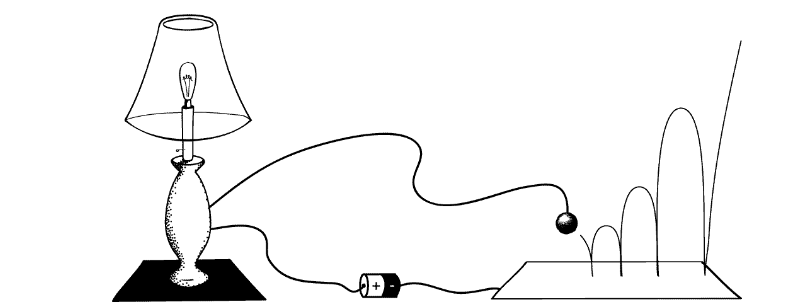
\includegraphics[width=\textwidth]{lamp.PNG}
        \caption{Benaceraff's solution to Thomson's lamp}
        \label{fig:my_label}
    \end{figure}
\end{frame}

\begin{frame}{The Last Thought Experiment}
    \begin{itemize}
        \item Imagine an urn with an infinite capacity and an infinite number of balls, each of them labelled with all the natural numbers from one to infinity.
    \end{itemize}
    
    \begin{figure}
        \centering
        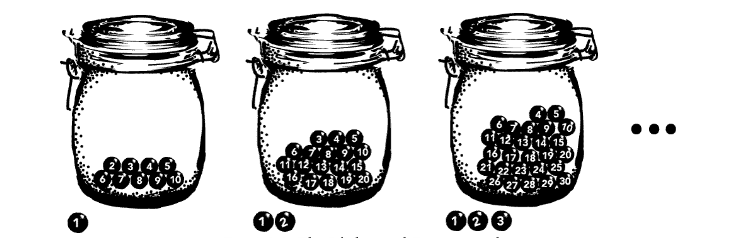
\includegraphics[width=\textwidth]{last.PNG}
        \caption{The Ross-Littlewood paradox}
        \label{fig:my_label}
    \end{figure}
\end{frame}

\begin{frame}{Final Thoughts}
    \begin{itemize}
        \item What was the reason for the creation of supertask?
        \item They are nothing more than mere intellectual and entertaining riddles which demonstrate humanity's ability to ask more questions than we can answer.
        \item This unending thirst for knowledge is what has fostered the growth of society and will continue to do so.
    \end{itemize}
\end{frame}

% Commands to include a figure:
%\begin{figure}
%\includegraphics[width=\textwidth]{your-figure's-file-name}
%\caption{\label{fig:your-figure}Caption goes here.}
%\end{figure}


\end{document}
